\chapter{Experimental Performance Evaluation or validation of solution}
\textit{This is a generic title. Replace it with an actual title that describes the context of the work.\\
Describe the  performance metrics, experimental hypotheses,  experimental conditions, test data, and expected results.  Provide the test data.  Interpret the results of the experiments.  Pay special attention to cases where the experiments give no information or did not come out as expected.  Draw lessons and conclusions from the experiments. Explain how additional experiments could validate or confirm results.}\\
\\
\\
\section{Hypothesis}
\begin{itemize}
	\item CS can be used to preserve image quality
	\item Can reduce dose and make a scalable algorithm
	\item SB can be implemented at ESRF
	\item Can use it on Bone data
\end{itemize}

\section{Data-set description}

\subsubsection{Data characteristics}
Parameters defining the projection file format

\begin{itemize}
	\item number of projections: 2000
	\item image dimensions: $2048 \times 20148$
	\item vertical and horizontal pixel size: 0.119865 microns
\end{itemize}

Parameters defining experiment

\begin{itemize}
	\item angle between projections: 0.09 degree
	\item Vertical rotation axis position: 1024.006591 pixel
	\item energy: 33.6
\end{itemize}

Parameters defining reconstruction

\begin{itemize}
	\item start voxel: (1,1,1) end voxel (2048, 2048, 256) of reconstruction volume
	\item Optic used: 0.119865	
	\item Pad method: reflect
	\item number of planes: 4
	\item number of angles: 645
	\item Rotation axis
\end{itemize}

\subsection{Sinograms and reconstruction}

\begin{figure}[ht!]
        \centering	
		\begin{subfigure}[b]{0.35\textwidth}
            \centering
            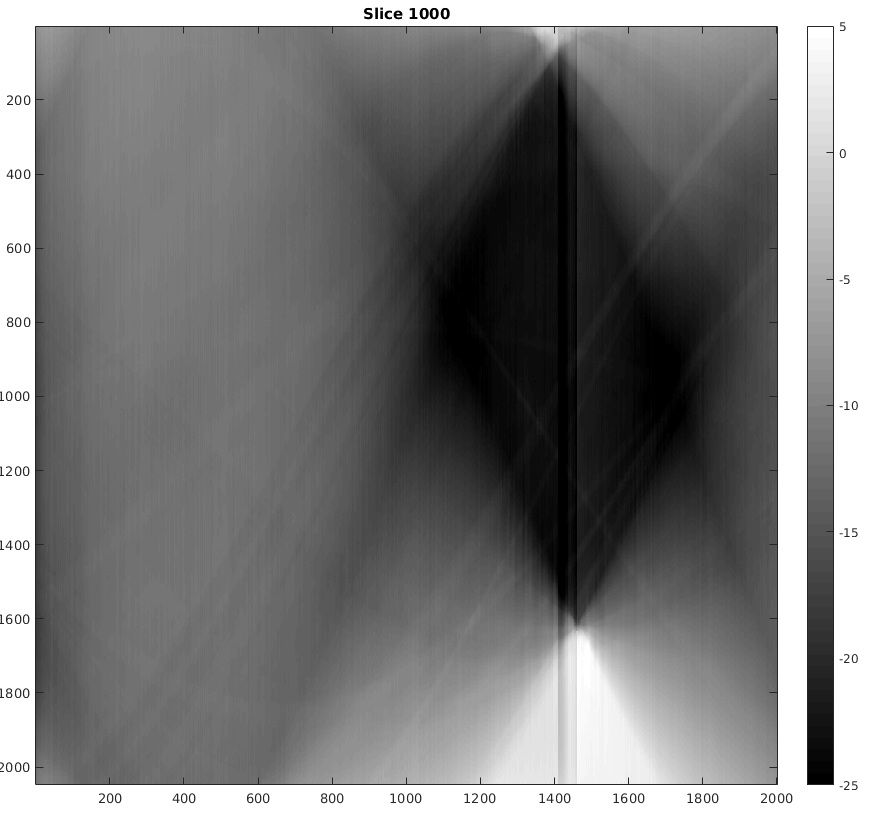
\includegraphics[width=\textwidth]{../Technical_Reports/Getting_familiarized_with_data/sinograms/Slice1000.png}
            %\caption[Network2]%
            %{{\small Network 1}}    
            \caption{One slice sinogram}
        \end{subfigure}
        \hfill
        \begin{subfigure}[b]{0.475\textwidth}  
            \centering 
            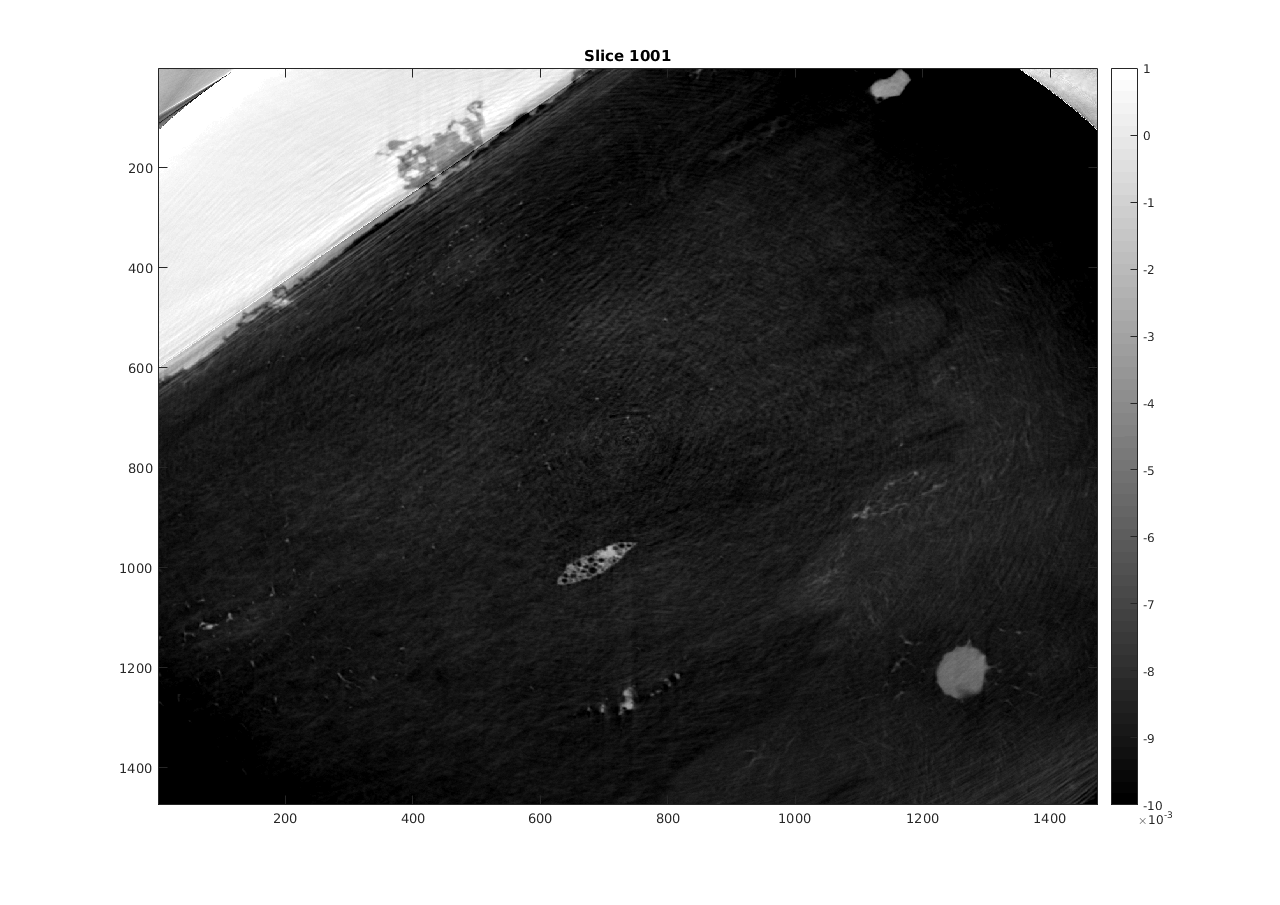
\includegraphics[width=\textwidth]{../Technical_Reports/Getting_familiarized_with_data/with0pad/slice1001.png}
            %\caption[]%
            %{{\small Network 2}}    
            \caption{One slice reconstruction}
        \end{subfigure}
        \caption{one slice of the 3D Micro SR-CT data used for the experiment}
\end{figure}

\section{Experiments description}
\subsection{Truncated images}
\begin{figure}[ht!]
        \centering	
		\begin{subfigure}[b]{0.30\textwidth}
            \centering
            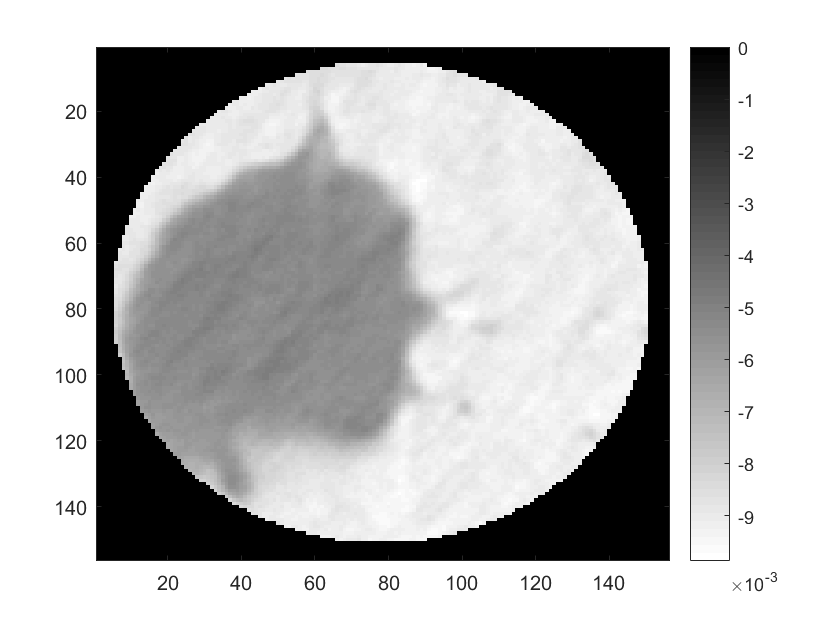
\includegraphics[width=\textwidth]{../../data/res/target1.png}
            %\caption[Network2]%
            %{{\small Network 1}}    
            \caption{Target 1}
        \end{subfigure}
        \hfill
        \begin{subfigure}[b]{0.30\textwidth}
            \centering
            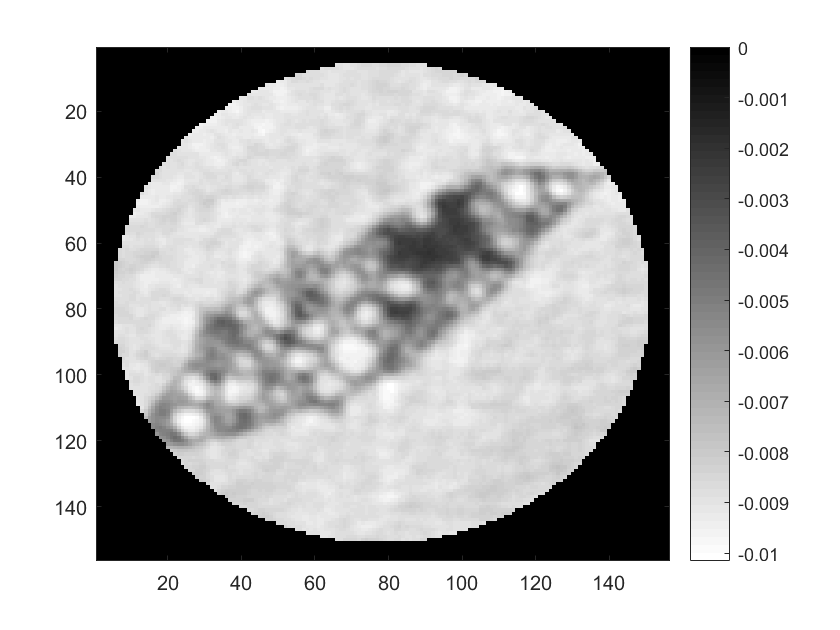
\includegraphics[width=\textwidth]{../../data/res/target2.png}
            %\caption[Network2]%
            %{{\small Network 1}}    
            \caption{Target 2}
        \end{subfigure}
        \hfill
        \begin{subfigure}[b]{0.30\textwidth}  
            \centering 
            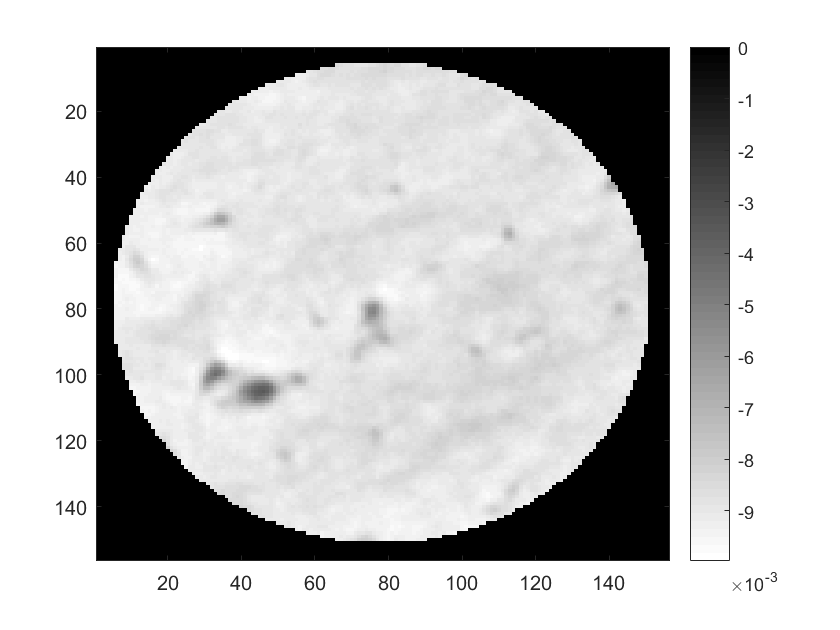
\includegraphics[width=\textwidth]{../../data/res/target3.png}
            %\caption[]%
            %{{\small Network 2}}    
            \caption{Target 3}
        \end{subfigure}
        \caption{Targets used for the Matlab experiments}
        \label{Fig:Targets}
\end{figure}

\subsection{Tunning of parameters}

\subsection{Scenarios}
Scenarios of Low dose on different targets were defined. The number of projections ranges from $1/2$ to $1/10$ of the number required for fully projected reconstruction.
An acquisition is considered fully projected when it generates $\pi / 2$ times the image size projections.\\
In our case we performed reconstruction with $1/2$, $1/4$, $1/7$ and $1/10$ of the projections. Knowing that our target images were of size $156 \times 156$ we used $125$, $63$, $36$, $25$ projections displayed in Figure\\% \ref{}. \\
These reconstructions were performed using FBP, SB-TV-2D and SB-TV-3D.

\section{Results}

These algorithms will be evaluated in terms of convergence of errors, visual comparison as well as the preservation of Edges and feature points of the resulted reconstructed image.\\
The errors are expressed in terms of mean squared error (MSE), peak signal to noise ration (PSNR) and total variation (TV), computed between the target image and the reconstructed image.\\
The Edge preservation will be evaluated in terms of total variation between the canny edge detection between the reference Target image and the reconstructed image.\\
The feature points were computed using SIFT algorithm for Scale-Invariant Transform Feature detection and description \cite{lowe04distinctive}. We decided to use SIFT algorithm because it is shift invariant and we noticed that if some edges were preserved, the smoothing imposed by the SB-TV reconstruction imposed some small shifting which can influence the total variation. Also it allows to display the eventual confusion of a post processing using edges in a intuitive way. The implementation of SIFT was performed by Vedaldi in matlab \cite{vedaldi2007open}.

\subsection{Error convergence}
\subsubsection{FBP}
	\begin{table}[ht!]
		\center
		\begin{tabular}{ | l || c | c | c | r | }
 			\hline			
   			\textbf{number of projections}	& \textbf{1/2}	& \textbf{1/4}	& \textbf{1/7}	& \textbf{1/10} \\
   			\hline
   			\hline
			\textbf{MSE}					& 6\%	& 7\%	& 9\%	& 11\% \\
			\hline  
			\textbf{PSNR}					& 67.90 & 66.92 & 64.17 & 62.21	\\
			\hline 
			\textbf{TV}						& 5.70  & 8.44  & 14.17 & 17.95 \\
			\hline
		\end{tabular}
		\caption{FBP Errors on Target 1}
		\label{tab:FBPErrorsTarget1}
		
	\end{table}

\subsubsection{SB-TV-2D}
\begin{figure}[ht!]
		
       		\centering
      		\begin{subfigure}[b]{0.475\textwidth}
            	\centering
            	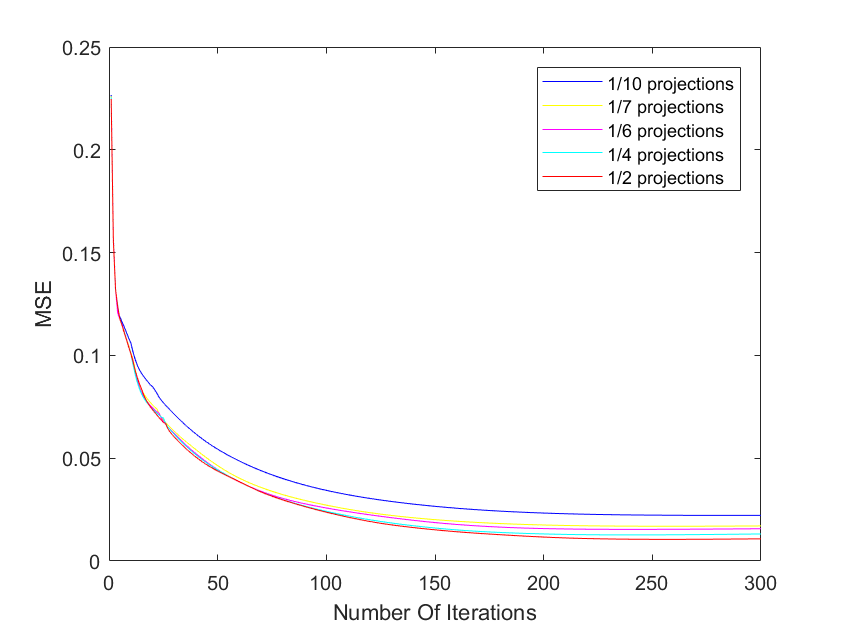
\includegraphics[width=\textwidth]{../../data/res/SB_Reconstruction/Errors/Err_MSE_2D_AllProj_Target1.png}
            	\caption{MSE}    
            	\label{subfig:Target1Fully}
        	\end{subfigure}
        	\hfill
        	\begin{subfigure}[b]{0.475\textwidth}  
            	\centering 
            	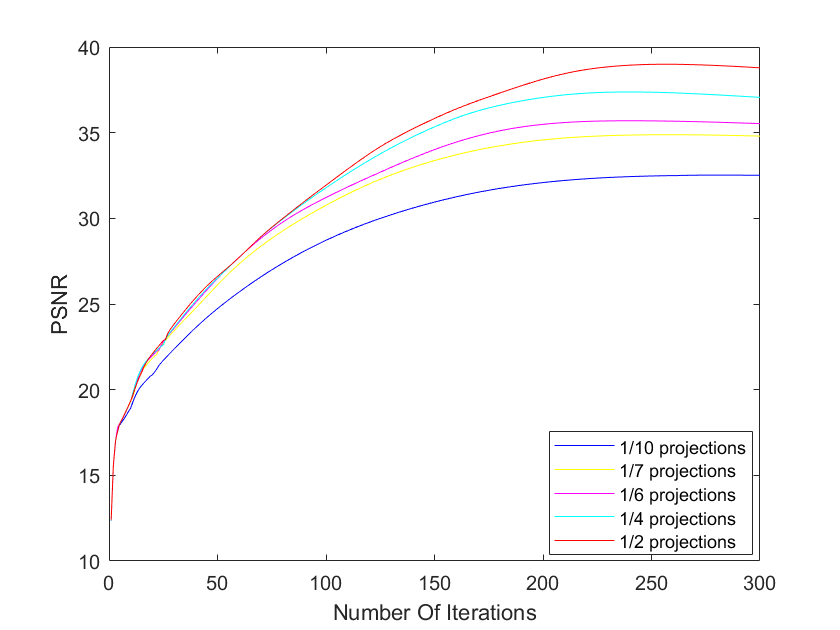
\includegraphics[width=\textwidth]{../../data/res/SB_Reconstruction/Errors/Err_PSNR_2D_AllProj_Target1.png}
            	\caption{PSNR}    
            	\label{subfig:FBP1Fully}
        	\end{subfigure}
        	\vskip\baselineskip
        	\begin{subfigure}[b]{0.475\textwidth}   
        	    \centering 
            	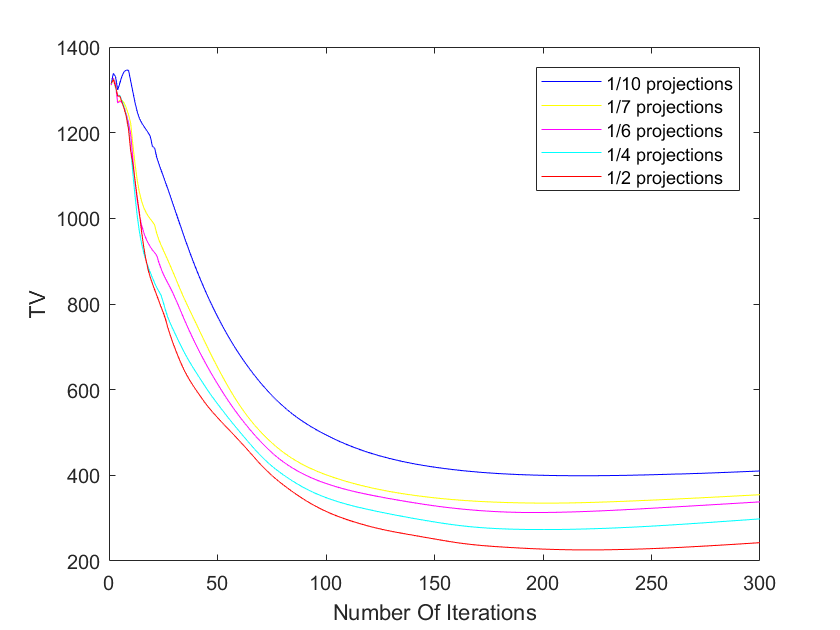
\includegraphics[width=\textwidth]{../../data/res/SB_Reconstruction/Errors/Err_TV_2D_AllProj_Target1.png}
            	\caption{TV}  
            	\label{subfig:20it1Fully}
        	\end{subfigure}
        	
        	\caption{SB-TV-2D errors on Target 1}
        	\label{fig:retFully}
    	\end{figure}


\subsubsection{SB-TV-3D}
\begin{figure}[ht!]
		
       		\centering
      		\begin{subfigure}[b]{0.475\textwidth}
            	\centering
            	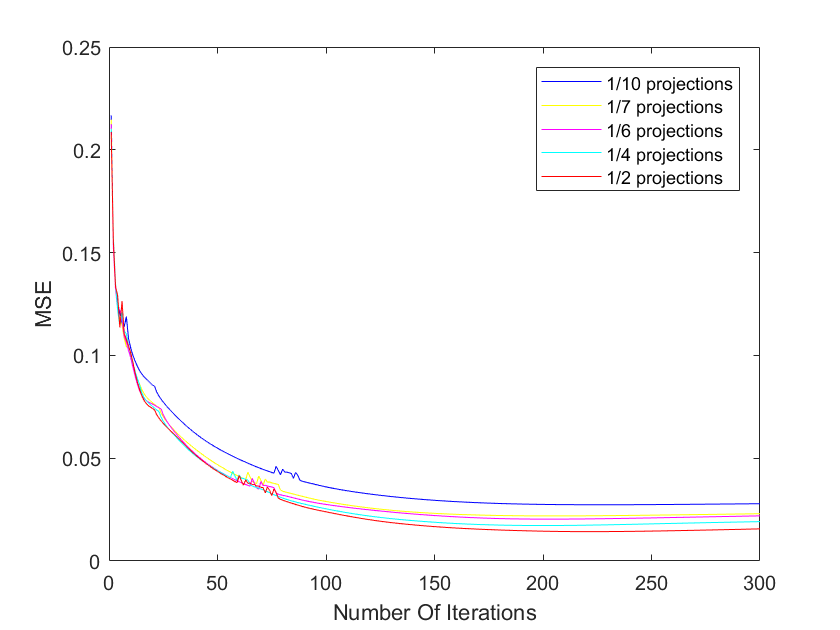
\includegraphics[width=\textwidth]{../../data/res/SB_Reconstruction/Errors/Err_MSE_3D_AllProj_Target1.png}
            	\caption{MSE}    
            	\label{subfig:Target1Fully3D}
        	\end{subfigure}
        	\hfill
        	\begin{subfigure}[b]{0.475\textwidth}  
            	\centering 
            	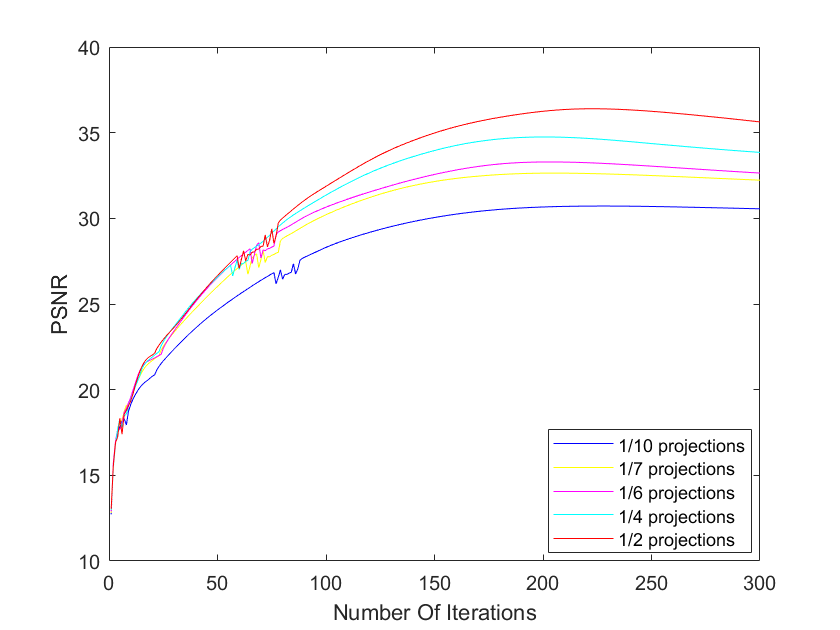
\includegraphics[width=\textwidth]{../../data/res/SB_Reconstruction/Errors/Err_PSNR_3D_AllProj_Target1.png}
            	\caption{PSNR}    
            	\label{subfig:FBP1Fully3D}
        	\end{subfigure}
        	\vskip\baselineskip
        	\begin{subfigure}[b]{0.475\textwidth}   
        	    \centering 
            	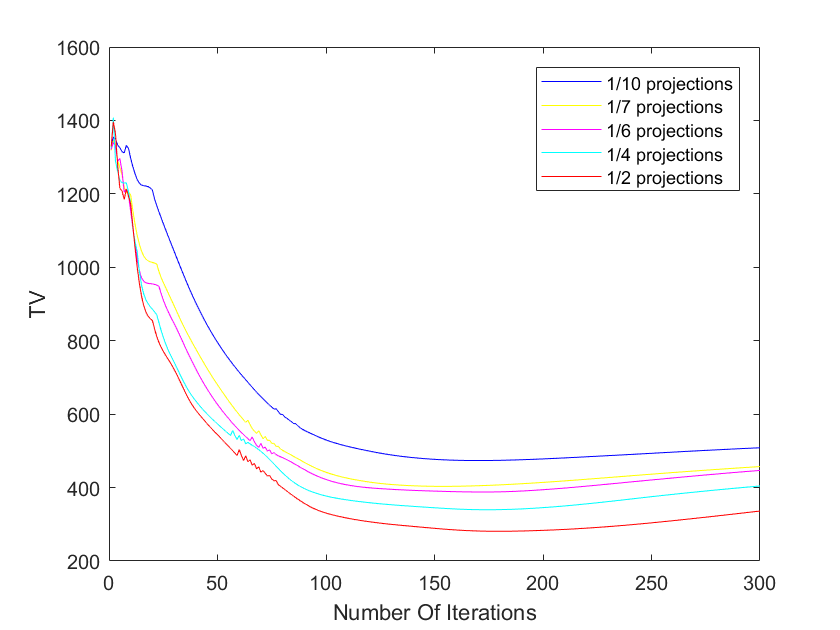
\includegraphics[width=\textwidth]{../../data/res/SB_Reconstruction/Errors/Err_TV_3D_AllProj_Target1.png}
            	\caption{TV}  
            	\label{subfig:20it1Fully3D}
        	\end{subfigure}
        	\caption{SB-TV-3D errors on Target 1}
        	\label{fig:retFully}
    	\end{figure}
\subsection{Visual comparison}

\begin{figure}[ht!]
       		\centering
      		\begin{subfigure}[b]{0.24\textwidth}
            	\centering
            	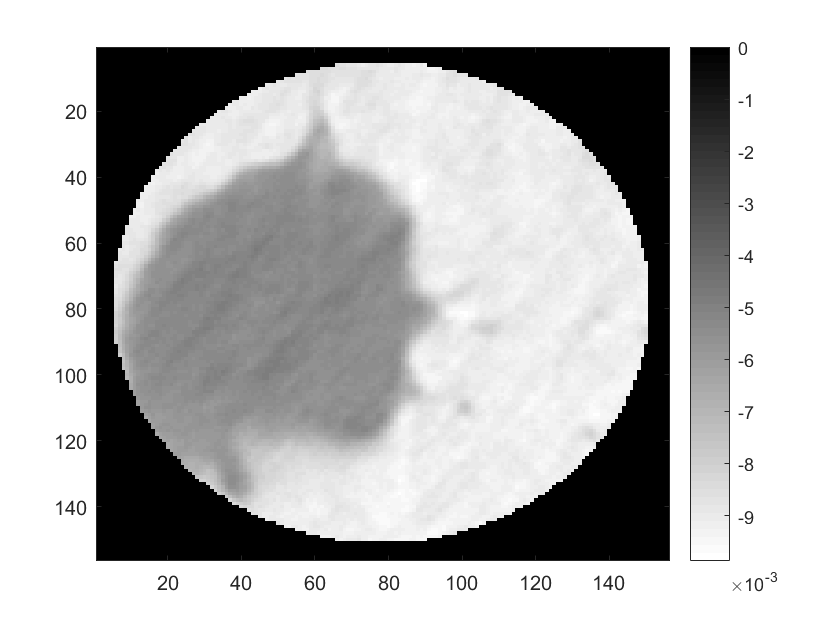
\includegraphics[width=\textwidth]{../../data/res/target1.png}
            	\caption{Target image}    
        	\end{subfigure}
        	%\hfill
        	\begin{subfigure}[b]{0.24\textwidth}  
            	\centering 
            	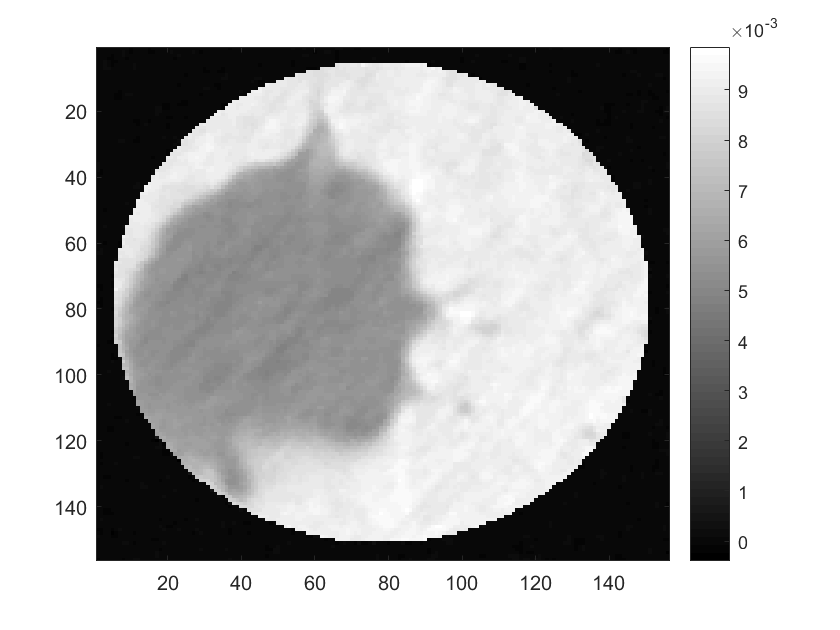
\includegraphics[width=\textwidth]{../../data/res/SB_Reconstruction/2D/Target1/1_2.png}
            	\caption{1/2 proj 2D}    
            	\label{subfig:156p1L-D}
        	\end{subfigure}
        	%\hfill
        	\begin{subfigure}[b]{0.24\textwidth}  
            	\centering 
            	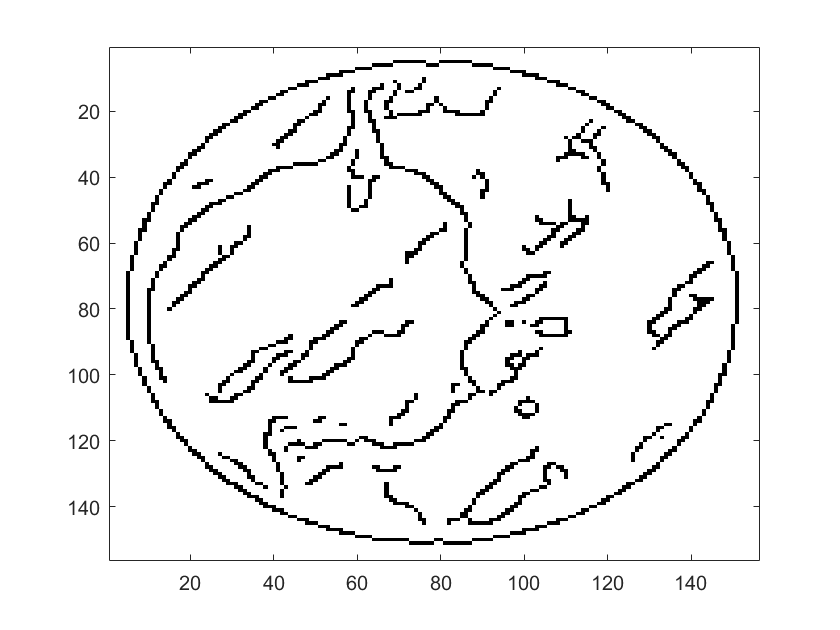
\includegraphics[width=\textwidth]{../../data/res/SB_Reconstruction/Edges/3D/it250_proj1_2.png}
            	\caption{1/2 proj 3D}    
            	\label{subfig:FBP1156p}
        	\end{subfigure}
        	%\hfill
        	\begin{subfigure}[b]{0.24\textwidth}  
            	\centering 
            	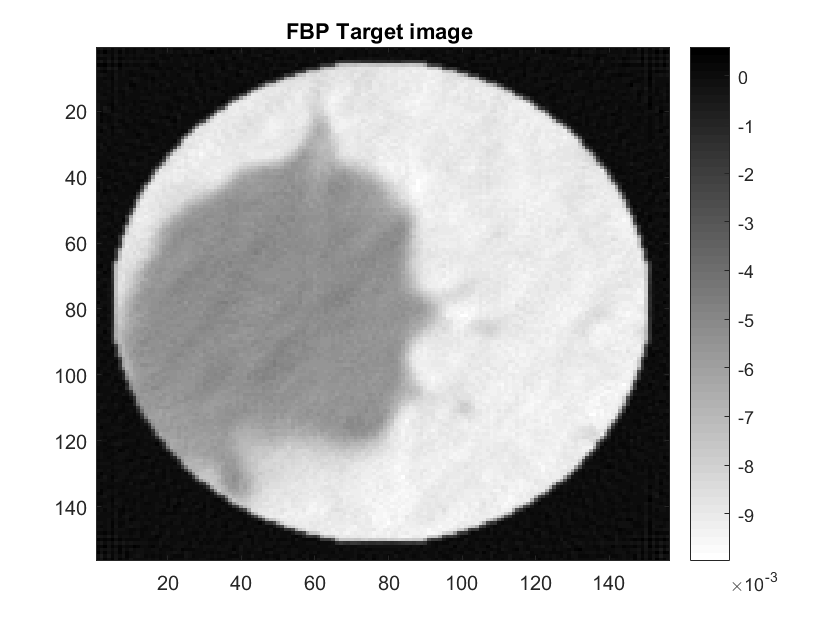
\includegraphics[width=\textwidth]{../../data/res/FBP/Target1/FBP_1_2_001_noise.png}
            	\caption{1/2 proj FBP}    
            	\label{subfig:FBP1156p}
        	\end{subfigure}
        	\vskip\baselineskip        	
        	      	        	
      		\begin{subfigure}[b]{0.24\textwidth}
            	\centering
            	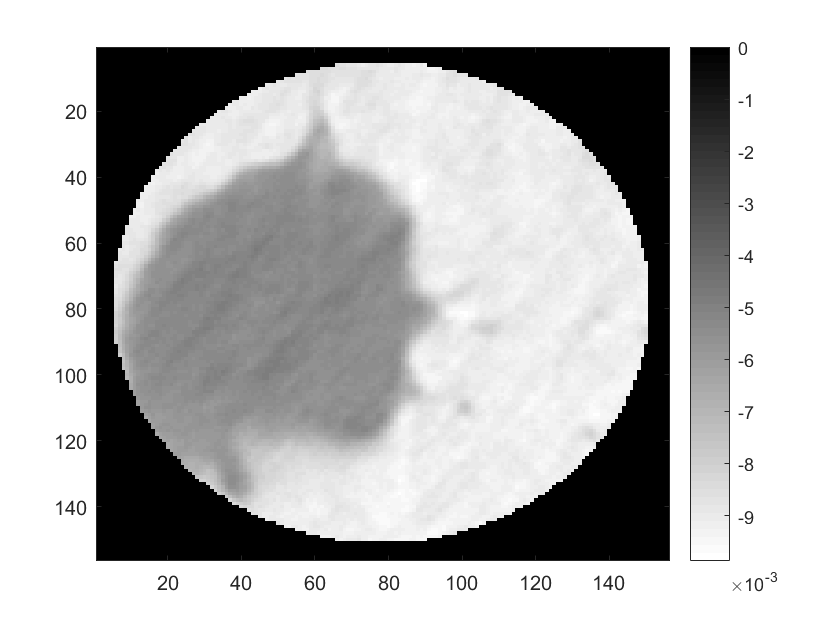
\includegraphics[width=\textwidth]{../../data/res/target1.png}
            	\caption{Target image}    
        	\end{subfigure}
        	%\hfill
        	\begin{subfigure}[b]{0.24\textwidth}  
            	\centering 
            	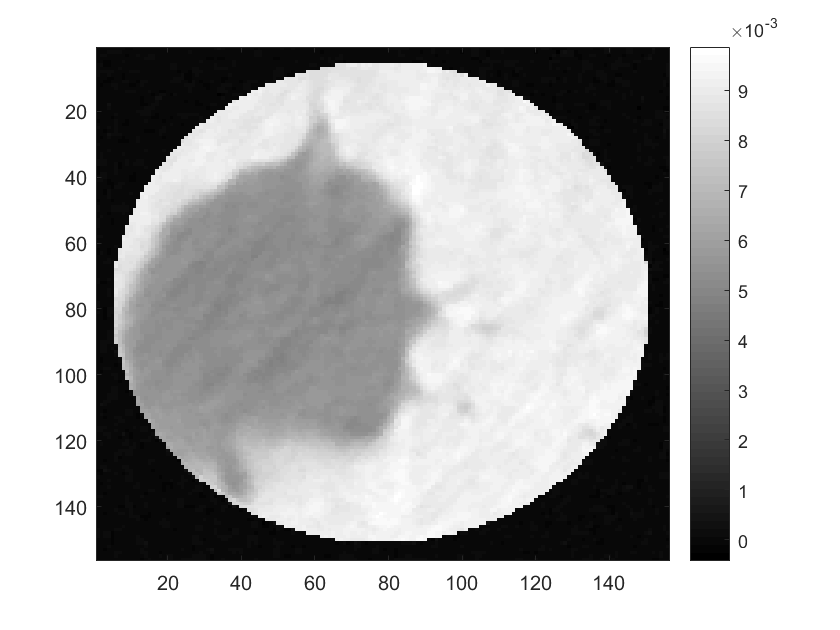
\includegraphics[width=\textwidth]{../../data/res/SB_Reconstruction/2D/Target1/1_4.png}
            	\caption{1/4 proj 2D}    
            	\label{subfig:156p1L-D}
        	\end{subfigure}
        	%\hfill
        	\begin{subfigure}[b]{0.24\textwidth}  
            	\centering 
            	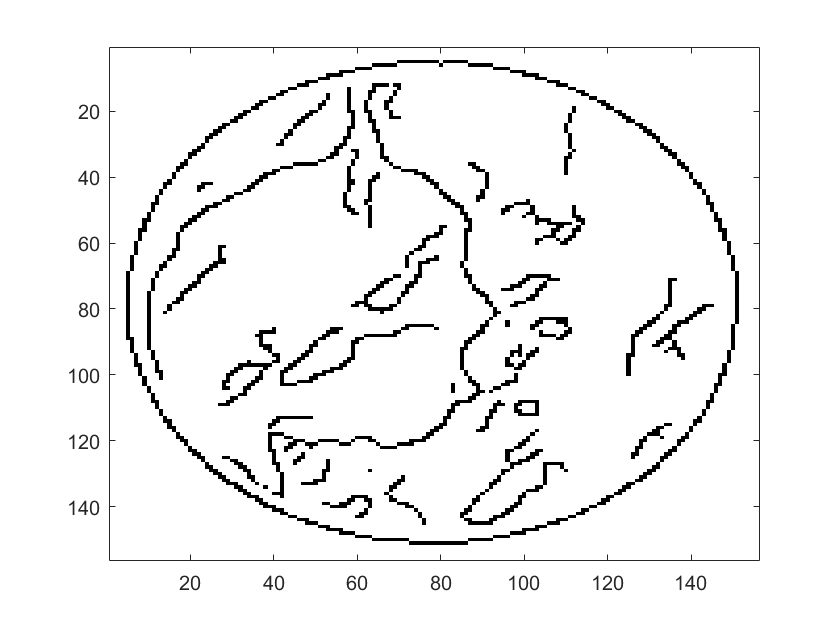
\includegraphics[width=\textwidth]{../../data/res/SB_Reconstruction/Edges/3D/it250_proj1_4.png}
            	\caption{1/4 proj 3D}    
            	\label{subfig:FBP1156p}
        	\end{subfigure}
        	%\hfill
        	\begin{subfigure}[b]{0.24\textwidth}  
            	\centering 
            	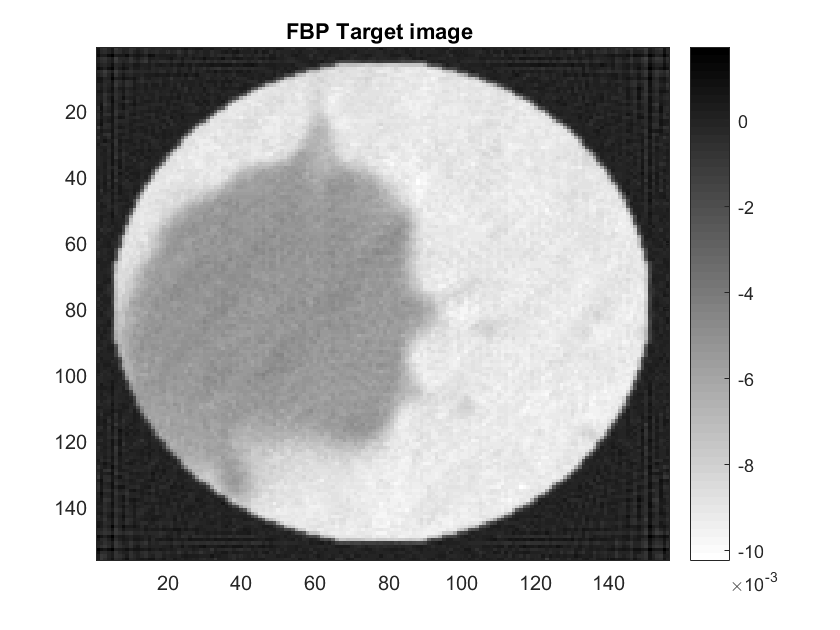
\includegraphics[width=\textwidth]{../../data/res/FBP/Target1/FBP_1_4_001_noise.png}
            	\caption{1/4 proj FBP}    
            	\label{subfig:FBP1156p}
        	\end{subfigure} 
        	\vskip\baselineskip        	
        	      	        	
      		\begin{subfigure}[b]{0.24\textwidth}
            	\centering
            	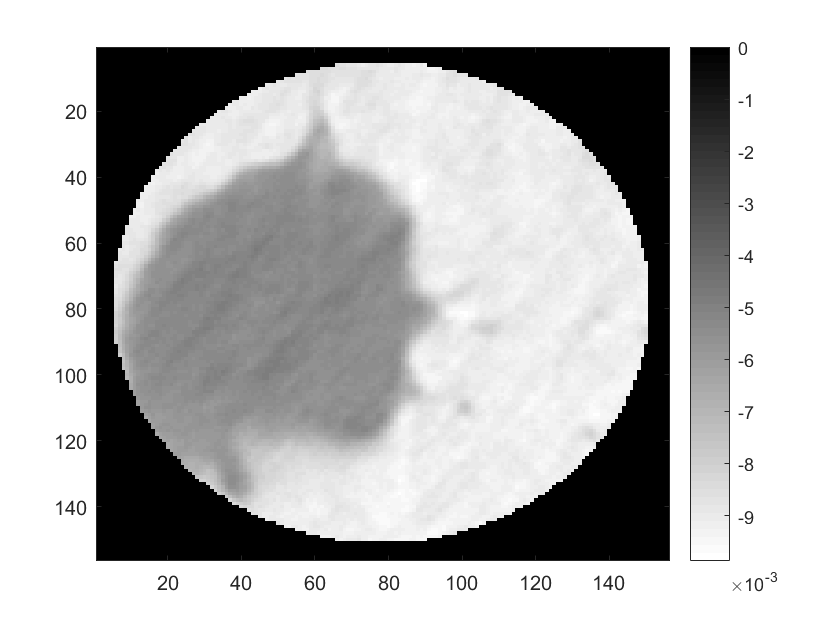
\includegraphics[width=\textwidth]{../../data/res/target1.png}
            	\caption{Target image}    
        	\end{subfigure}
        	%\hfill
        	\begin{subfigure}[b]{0.24\textwidth}  
            	\centering 
            	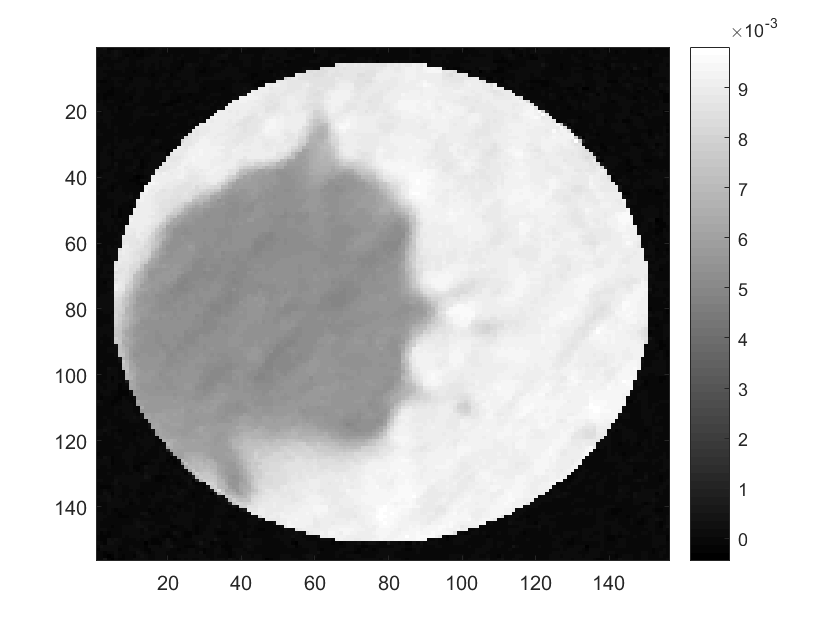
\includegraphics[width=\textwidth]{../../data/res/SB_Reconstruction/2D/Target1/1_7.png}
            	\caption{1/7 proj 2D}    
            	\label{subfig:156p1L-D}
        	\end{subfigure}
        	%\hfill
        	\begin{subfigure}[b]{0.24\textwidth}  
            	\centering 
            	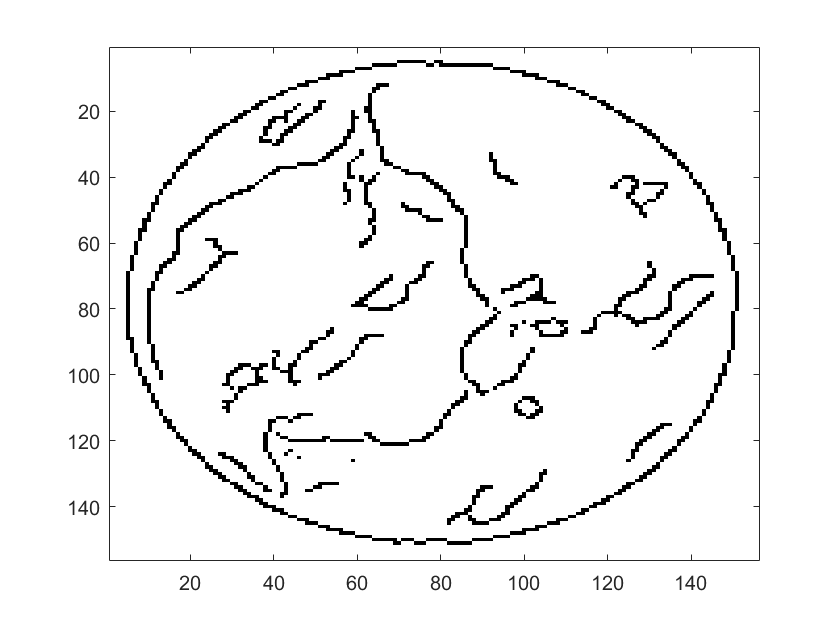
\includegraphics[width=\textwidth]{../../data/res/SB_Reconstruction/Edges/3D/it250_proj1_7.png}
            	\caption{1/7 proj 3D}    
            	\label{subfig:FBP1156p}
        	\end{subfigure}
        	%\hfill
        	\begin{subfigure}[b]{0.24\textwidth}  
            	\centering 
            	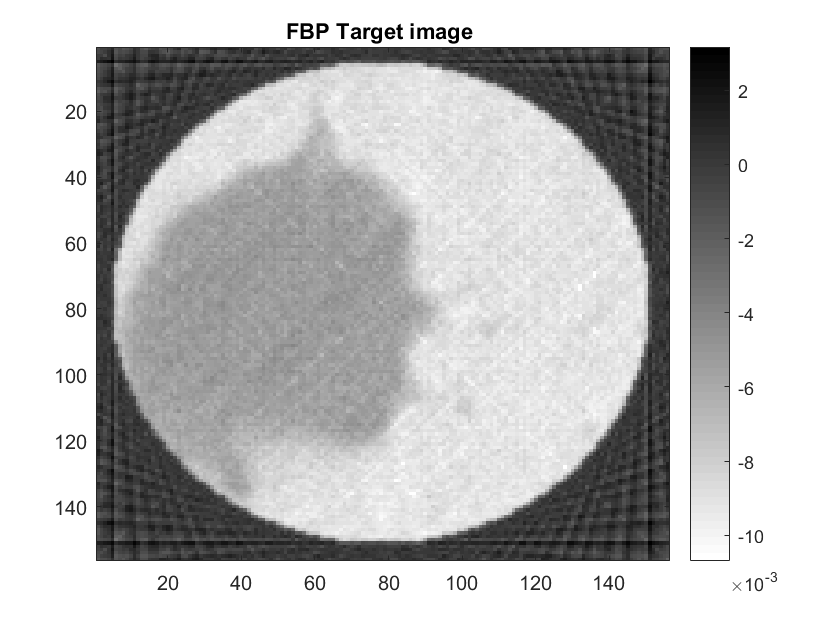
\includegraphics[width=\textwidth]{../../data/res/FBP/Target1/FBP_1_7_001_noise.png}
            	\caption{1/7 proj FBP}    
            	\label{subfig:FBP1156p}
        	\end{subfigure}
        	
        	\vskip\baselineskip        	
        	      	        	
      		\begin{subfigure}[b]{0.24\textwidth}
            	\centering
            	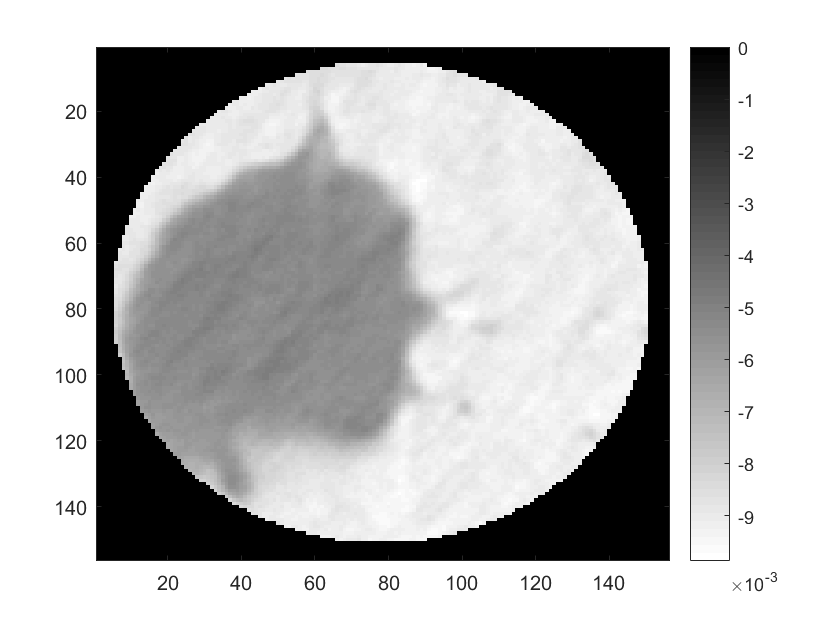
\includegraphics[width=\textwidth]{../../data/res/target1.png}
            	\caption{Target image}    
        	\end{subfigure}
        	%\hfill
        	\begin{subfigure}[b]{0.24\textwidth}  
            	\centering 
            	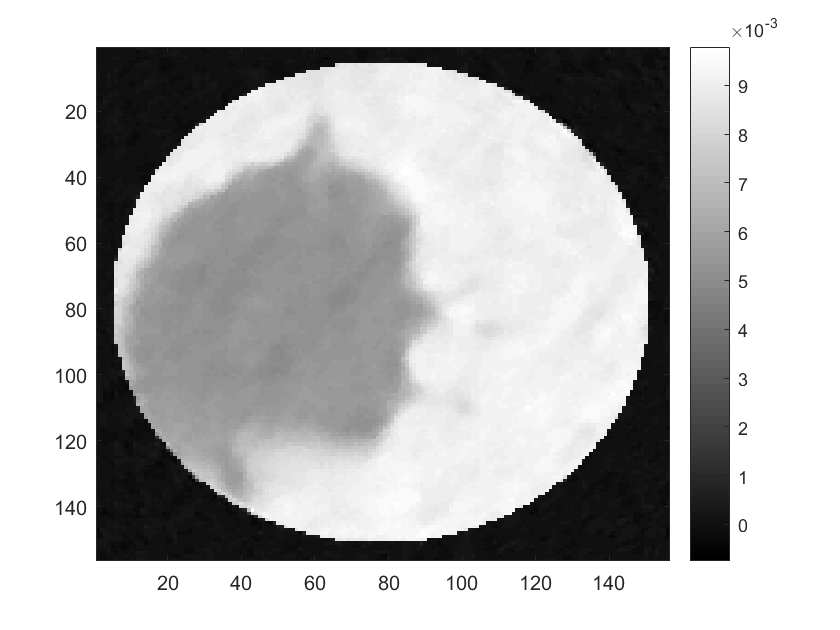
\includegraphics[width=\textwidth]{../../data/res/SB_Reconstruction/2D/Target1/1_10.png}
            	\caption{1/10 proj 2D}    
            	\label{subfig:156p1L-D}
        	\end{subfigure}
        	%\hfill
        	\begin{subfigure}[b]{0.24\textwidth}  
            	\centering 
            	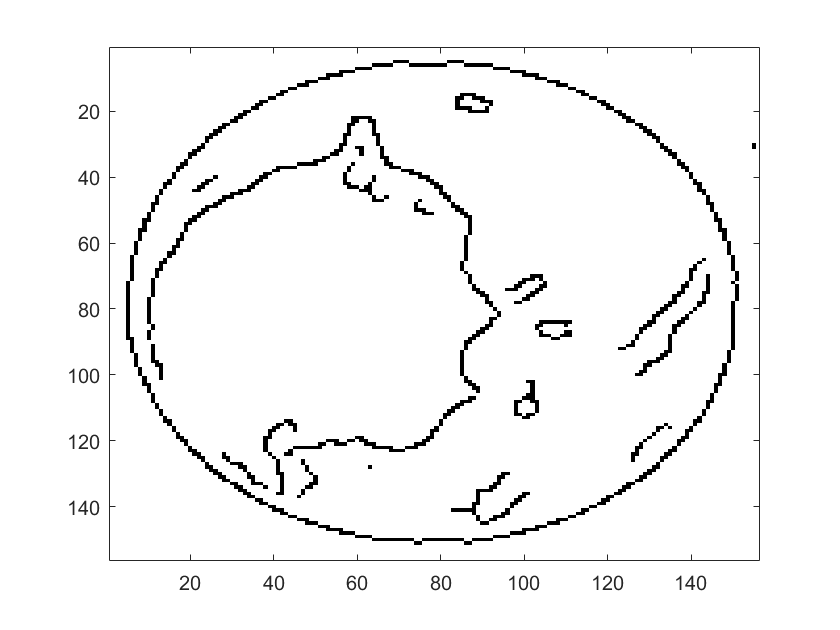
\includegraphics[width=\textwidth]{../../data/res/SB_Reconstruction/Edges/3D/it250_proj1_10.png}
            	\caption{1/10 proj 3D}    
            	\label{subfig:FBP1156p}
        	\end{subfigure}
        	%\hfill
        	\begin{subfigure}[b]{0.24\textwidth}  
            	\centering 
            	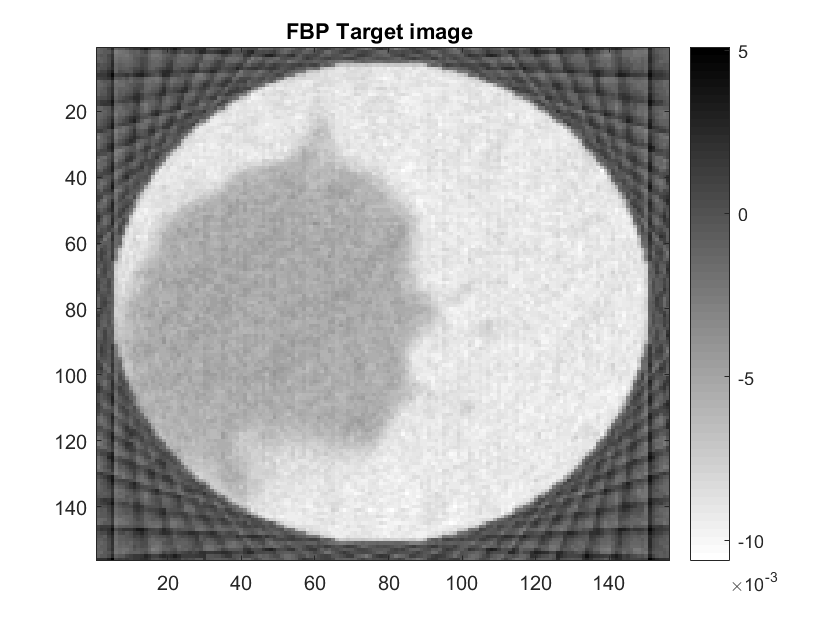
\includegraphics[width=\textwidth]{../../data/res/FBP/Target1/FBP_1_10_001_noise.png}
            	\caption{1/10 proj FBP}    
            	\label{subfig:FBP1156p}
        	\end{subfigure}
        	\caption{Canny edge detection}
        	\label{fig:Canny}
    	\end{figure}


\subsection{Edges preservation}


\begin{figure}[ht!]
       		\centering
      		\begin{subfigure}[b]{0.24\textwidth}
            	\centering
            	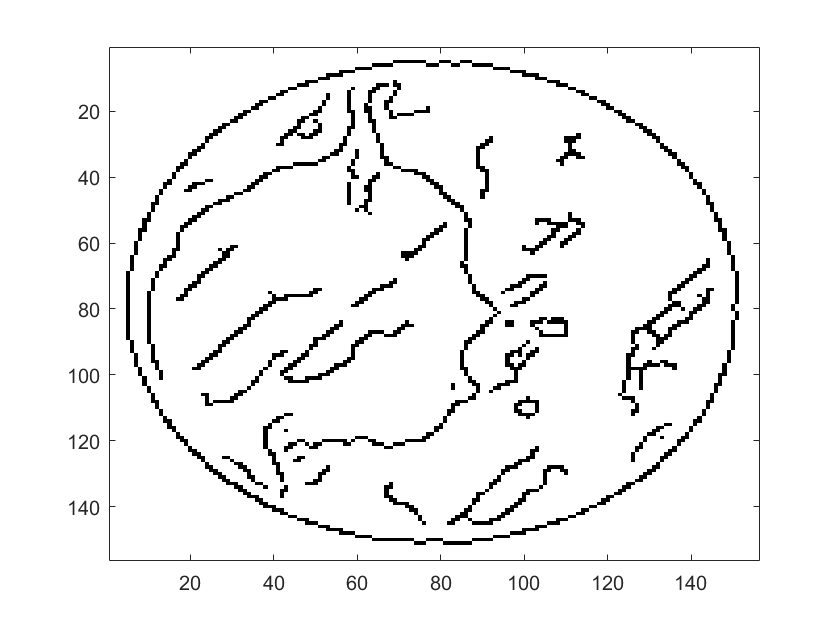
\includegraphics[width=\textwidth]{../../data/res/target1_edges.png}
            	\caption{Target image}    
        	\end{subfigure}
        	%\hfill
        	\begin{subfigure}[b]{0.24\textwidth}  
            	\centering 
            	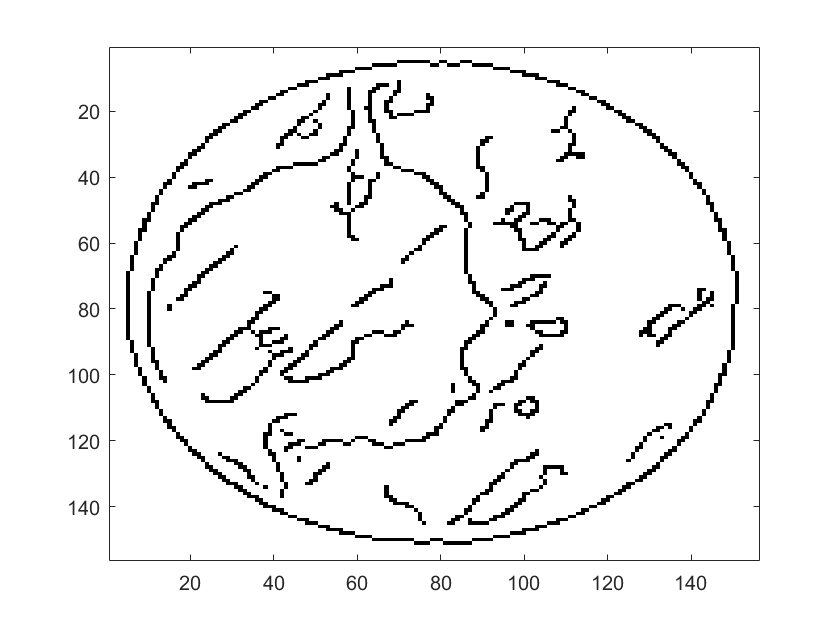
\includegraphics[width=\textwidth]{../../data/res/SB_Reconstruction/Edges/2D/it250_proj1_2.png}
            	\caption{1/2 proj 2D}    
            	\label{subfig:156p1L-D}
        	\end{subfigure}
        	%\hfill
        	\begin{subfigure}[b]{0.24\textwidth}  
            	\centering 
            	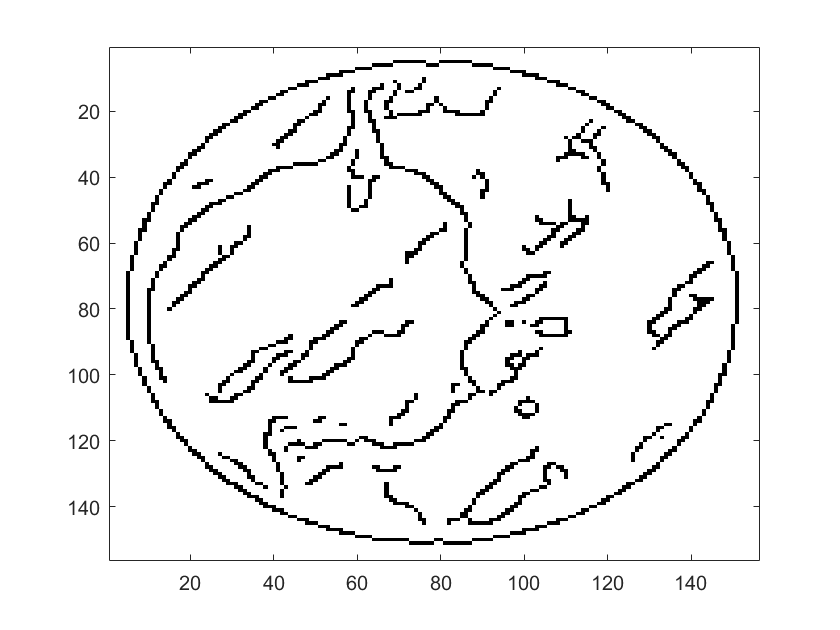
\includegraphics[width=\textwidth]{../../data/res/SB_Reconstruction/Edges/3D/it250_proj1_2.png}
            	\caption{1/2 proj 3D}    
            	\label{subfig:FBP1156p}
        	\end{subfigure}
        	%\hfill
        	\begin{subfigure}[b]{0.24\textwidth}  
            	\centering 
            	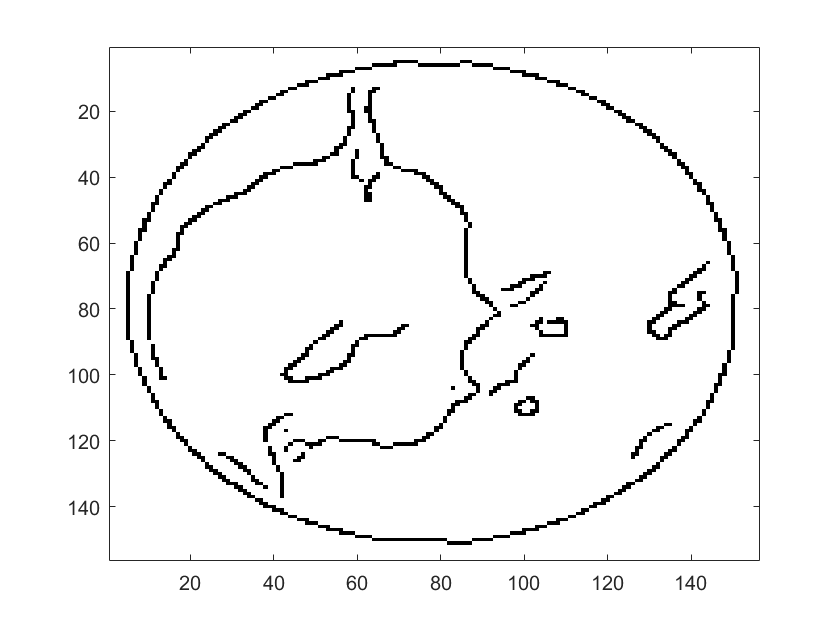
\includegraphics[width=\textwidth]{../../data/res/FBP/Edges/proj_1_2.png}
            	\caption{1/2 proj FBP}    
            	\label{subfig:FBP1156p}
        	\end{subfigure}
        	\vskip\baselineskip        	
        	      	        	
      		\begin{subfigure}[b]{0.24\textwidth}
            	\centering
            	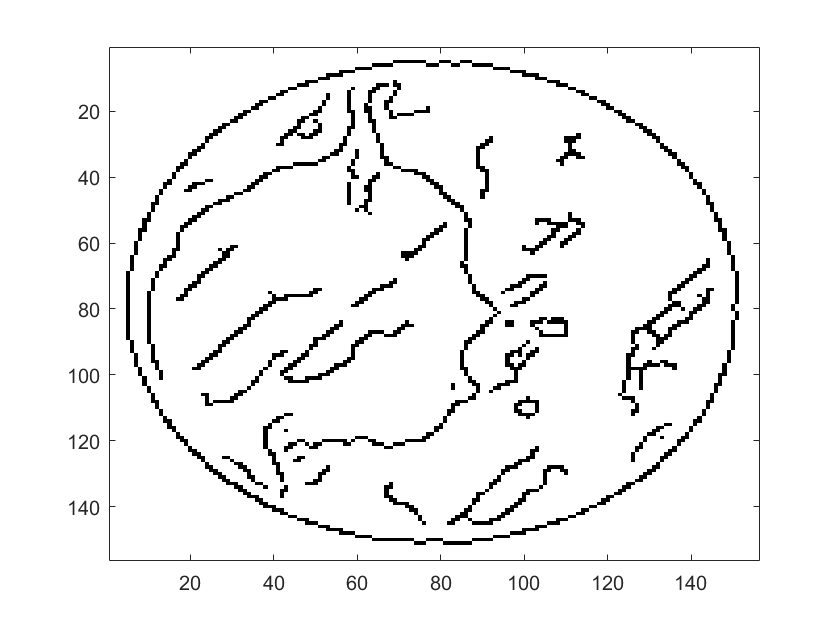
\includegraphics[width=\textwidth]{../../data/res/target1_edges.png}
            	\caption{Target image}    
        	\end{subfigure}
        	%\hfill
        	\begin{subfigure}[b]{0.24\textwidth}  
            	\centering 
            	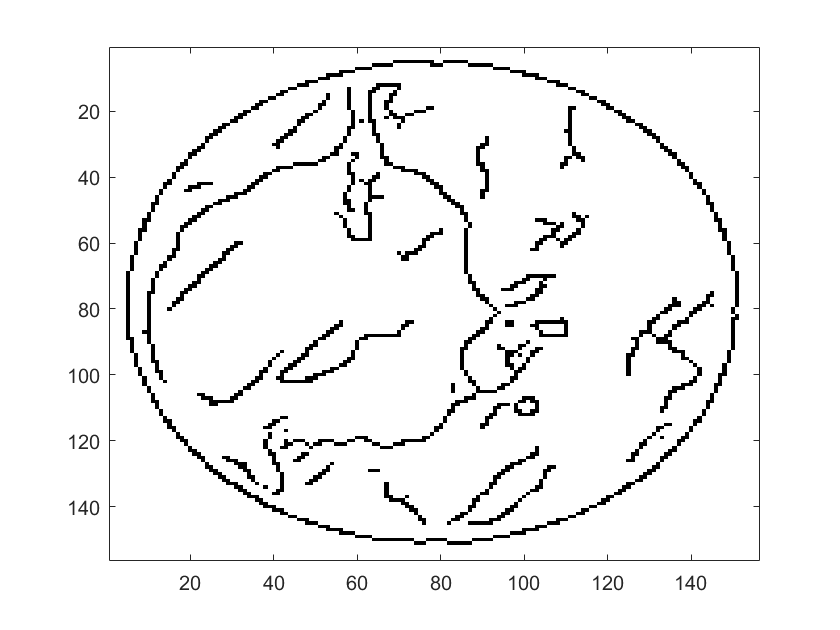
\includegraphics[width=\textwidth]{../../data/res/SB_Reconstruction/Edges/2D/it250_proj1_4.png}
            	\caption{1/4 proj 2D}    
            	\label{subfig:156p1L-D}
        	\end{subfigure}
        	%\hfill
        	\begin{subfigure}[b]{0.24\textwidth}  
            	\centering 
            	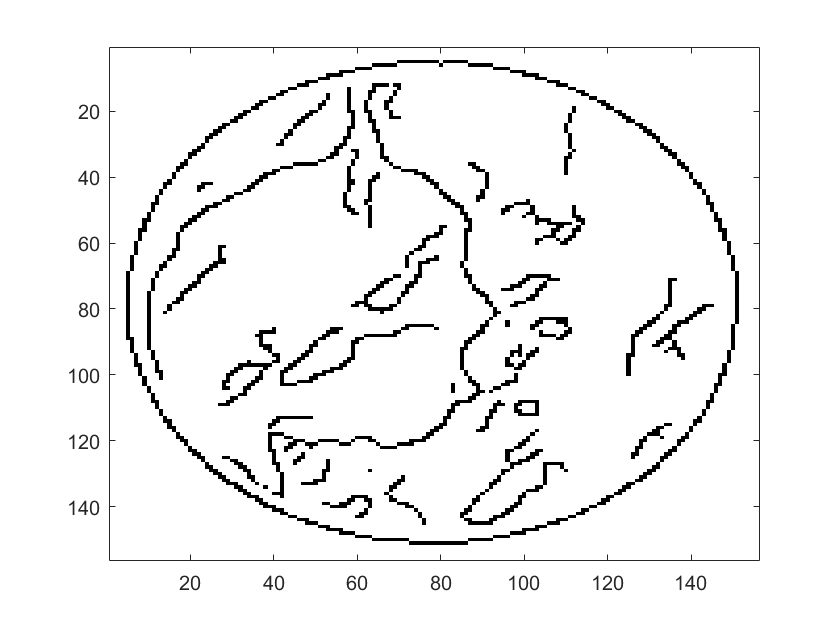
\includegraphics[width=\textwidth]{../../data/res/SB_Reconstruction/Edges/3D/it250_proj1_4.png}
            	\caption{1/4 proj 3D}    
            	\label{subfig:FBP1156p}
        	\end{subfigure}
        	%\hfill
        	\begin{subfigure}[b]{0.24\textwidth}  
            	\centering 
            	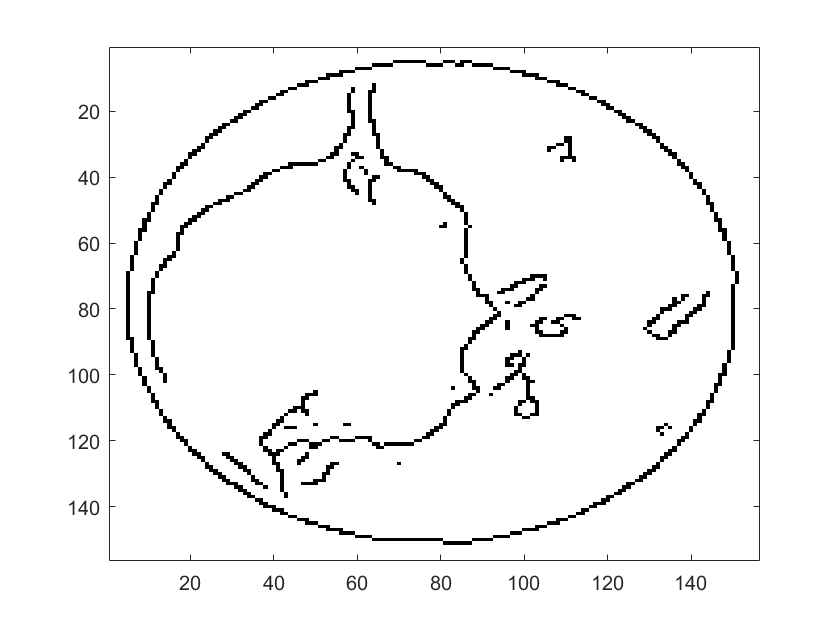
\includegraphics[width=\textwidth]{../../data/res/FBP/Edges/proj_1_4.png}
            	\caption{1/4 proj FBP}    
            	\label{subfig:FBP1156p}
        	\end{subfigure} 
        	\vskip\baselineskip        	
        	      	        	
      		\begin{subfigure}[b]{0.24\textwidth}
            	\centering
            	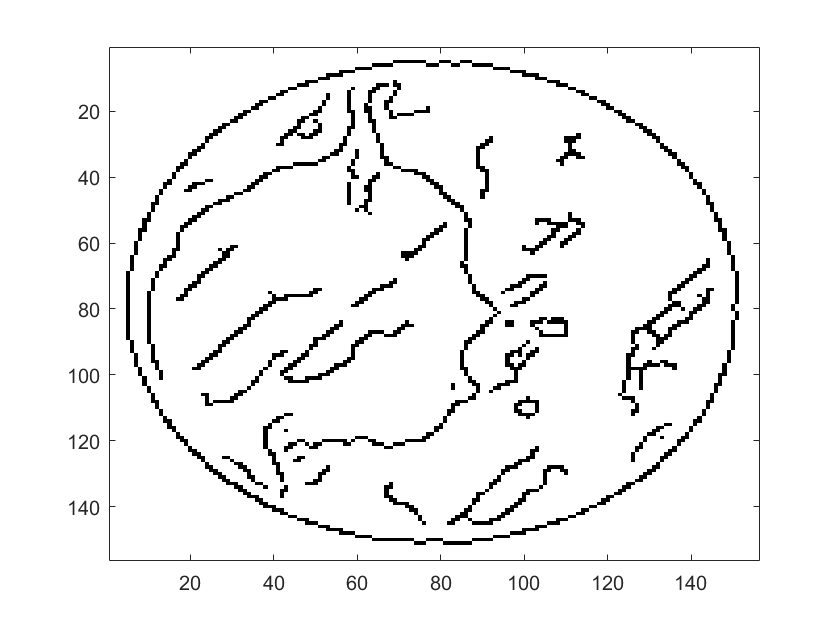
\includegraphics[width=\textwidth]{../../data/res/target1_edges.png}
            	\caption{Target image}    
        	\end{subfigure}
        	%\hfill
        	\begin{subfigure}[b]{0.24\textwidth}  
            	\centering 
            	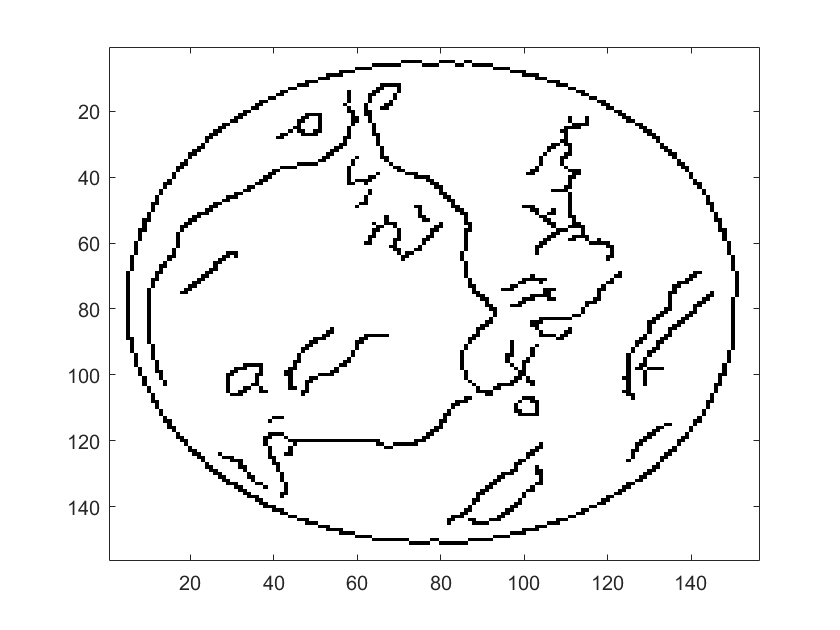
\includegraphics[width=\textwidth]{../../data/res/SB_Reconstruction/Edges/2D/it250_proj1_7.png}
            	\caption{1/7 proj 2D}    
            	\label{subfig:156p1L-D}
        	\end{subfigure}
        	%\hfill
        	\begin{subfigure}[b]{0.24\textwidth}  
            	\centering 
            	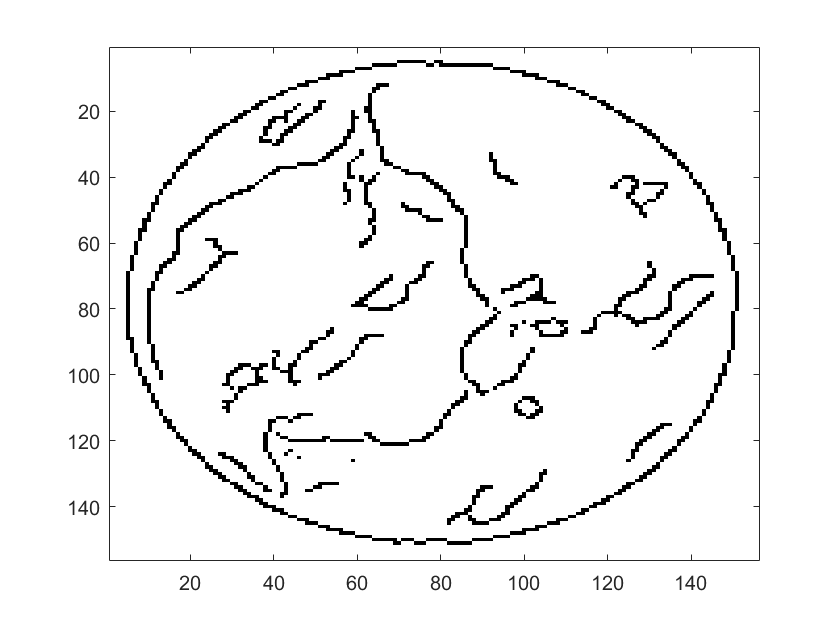
\includegraphics[width=\textwidth]{../../data/res/SB_Reconstruction/Edges/3D/it250_proj1_7.png}
            	\caption{1/7 proj 3D}    
            	\label{subfig:FBP1156p}
        	\end{subfigure}
        	%\hfill
        	\begin{subfigure}[b]{0.24\textwidth}  
            	\centering 
            	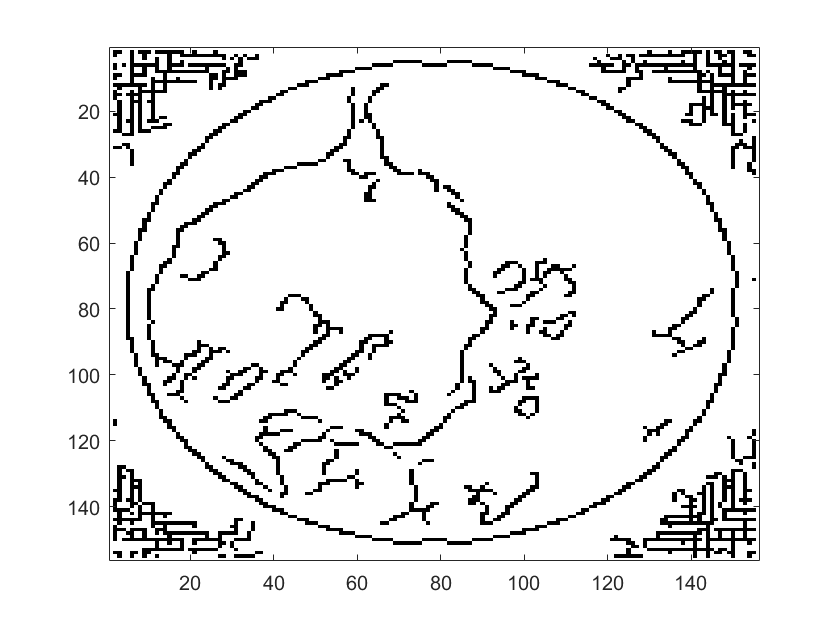
\includegraphics[width=\textwidth]{../../data/res/FBP/Edges/proj_1_7.png}
            	\caption{1/7 proj FBP}    
            	\label{subfig:FBP1156p}
        	\end{subfigure}
        	
        	\vskip\baselineskip        	
        	      	        	
      		\begin{subfigure}[b]{0.24\textwidth}
            	\centering
            	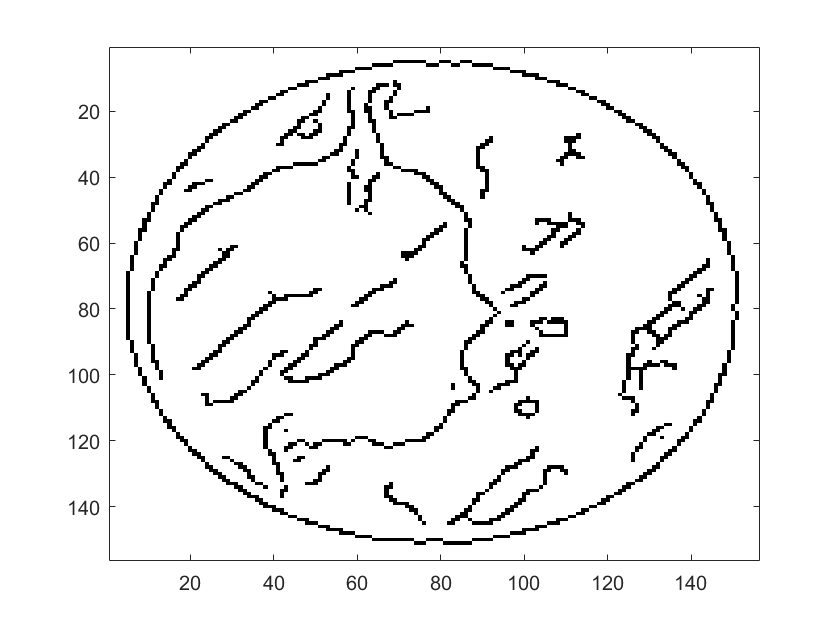
\includegraphics[width=\textwidth]{../../data/res/target1_edges.png}
            	\caption{Target image}    
        	\end{subfigure}
        	%\hfill
        	\begin{subfigure}[b]{0.24\textwidth}  
            	\centering 
            	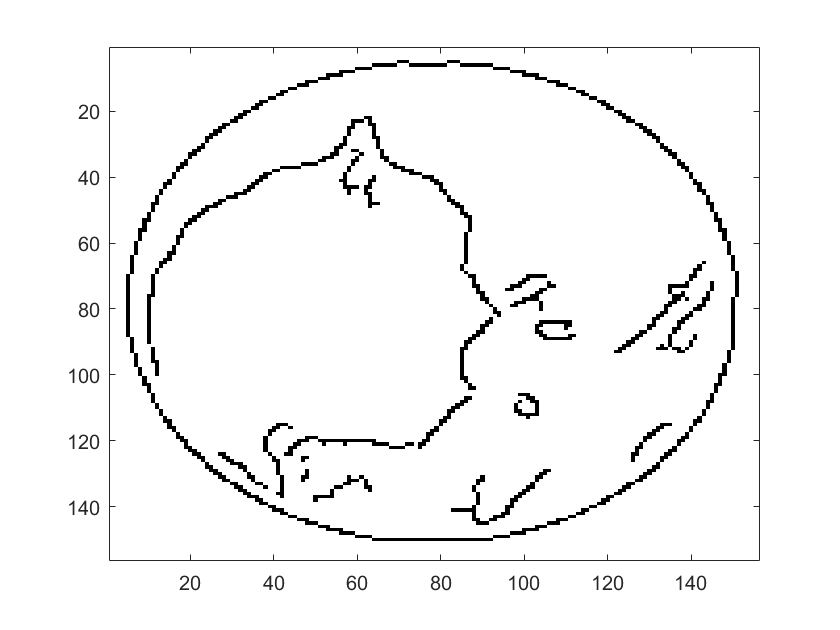
\includegraphics[width=\textwidth]{../../data/res/SB_Reconstruction/Edges/2D/it250_proj1_10.png}
            	\caption{1/10 proj 2D}    
            	\label{subfig:156p1L-D}
        	\end{subfigure}
        	%\hfill
        	\begin{subfigure}[b]{0.24\textwidth}  
            	\centering 
            	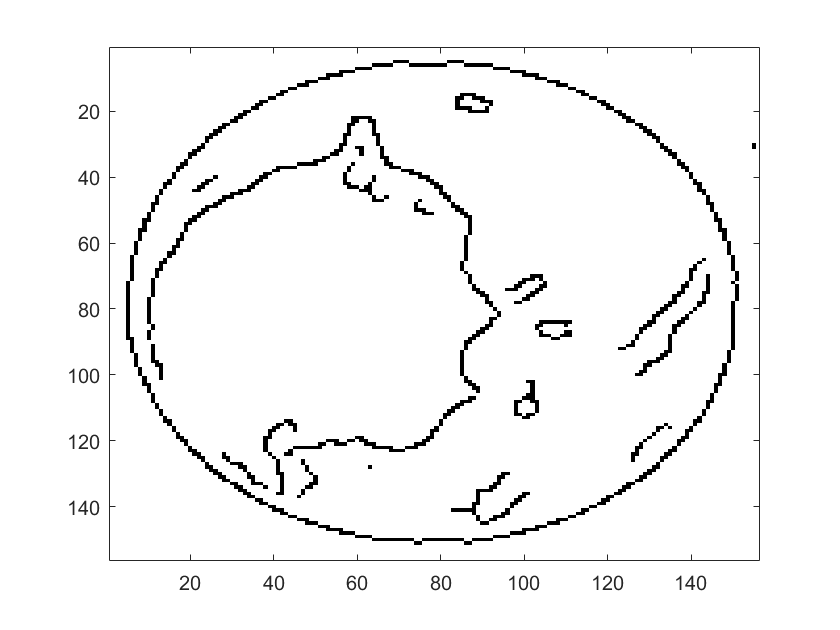
\includegraphics[width=\textwidth]{../../data/res/SB_Reconstruction/Edges/3D/it250_proj1_10.png}
            	\caption{1/10 proj 3D}    
            	\label{subfig:FBP1156p}
        	\end{subfigure}
        	%\hfill
        	\begin{subfigure}[b]{0.24\textwidth}  
            	\centering 
            	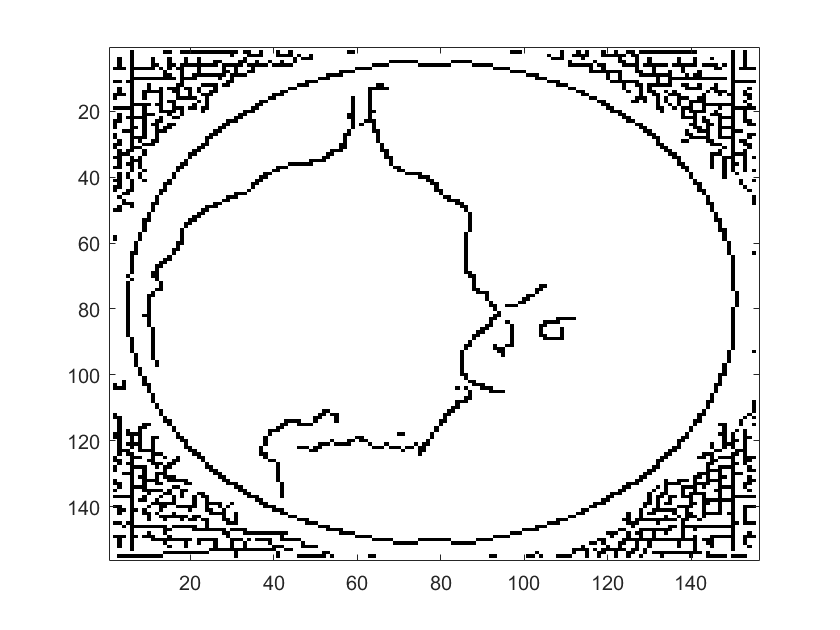
\includegraphics[width=\textwidth]{../../data/res/FBP/Edges/proj_1_10.png}
            	\caption{1/10 proj FBP}    
            	\label{subfig:FBP1156p}
        	\end{subfigure}
        	\caption{Canny edge detection}
        	\label{fig:Canny}
    	\end{figure}


\subsection{Feature points preservation}

\begin{itemize}
	\item show images compare to FBP
	\item computation time
	\item error rates
	\item compare corronal sagital and axial views
	\item 3D not as good as expected? Why? How to make ferther tests to understand why?
\end{itemize}
